\documentclass{beamer}
%
% Choose how your presentation looks.
%
% For more themes, color themes and font themes, see:
% http://deic.uab.es/~iblanes/beamer_gallery/index_by_theme.html
%
\mode<presentation>
{
  \usetheme{default}      % or try Darmstadt, Madrid, Warsaw, ...
  \usecolortheme{default} % or try albatross, beaver, crane, ...
  \usefonttheme{default}  % or try serif, structurebold, ...
  \setbeamertemplate{navigation symbols}{}
  \setbeamertemplate{caption}[numbered]
  \setbeamertemplate{footline}[frame number]
  \setbeamertemplate{itemize items}[circle]
  \setbeamertemplate{theorems}[numbered]
  \setbeamercolor*{structure}{bg=white,fg=blue}
  \setbeamerfont{block title}{size=\normalsize}
}

\newtheorem{proposition}[theorem]{Proposition}
\theoremstyle{definition}
\newtheorem{algorithm}[theorem]{Algorithm}
\newtheorem{idea}[theorem]{Idea}

\usepackage[english]{babel}
\usepackage[utf8]{inputenc}
\usepackage[T1]{fontenc}
\usepackage{aligned-overset}
\usepackage{alltt}
\usepackage{amsmath}
\usepackage{csquotes}
\usepackage{multicol}
\usepackage{stmaryrd}
\usepackage{tabularx}

\renewcommand\tabularxcolumn[1]{m{#1}}
\newcolumntype{R}{>{\raggedleft\arraybackslash}X}

\usepackage{pgfplots, pgfplotstable}
\pgfplotsset{compat=1.15}
\pgfplotstableread[col sep=comma,]{data.csv}\datatable

\def\code#1{\texttt{\frenchspacing#1}}
\def\padding{\vspace{0.5cm}}
\def\spadding{\vspace{0.25cm}}
\def\b{\textcolor{blue}}
\def\r{\textcolor{red}}
\def\g#1{{\usebeamercolor[fg]{block title example}{#1}}}

% fix for \pause in align
\makeatletter
\let\save@measuring@true\measuring@true
\def\measuring@true{%
  \save@measuring@true
  \def\beamer@sortzero##1{\beamer@ifnextcharospec{\beamer@sortzeroread{##1}}{}}%
  \def\beamer@sortzeroread##1<##2>{}%
  \def\beamer@finalnospec{}%
}
\makeatother

\usepackage[sorting=ynt,style=numeric]{biblatex}
\addbibresource{sources.bib}

\title{TypeScript: Final Report \\[0.1cm] \small{Practical Course: Contributing to an Open-Source Project}}
\author{Jonas Hübotter}
\date{March 16, 2021}

\begin{document}

\begin{frame}
  \titlepage
\end{frame}

\begin{frame}{Outline}
 \tableofcontents
\end{frame}

\section{TypeScript revisted}
\begin{frame}{TypeScript revisited}
TypeScript is
\begin{itemize}
    \item a programming language\pause;
    \item a superset of JavaScript\pause;
    \item a transpiler\pause;
    \item a static type system\pause;
    \item funded and developed by Microsoft\pause;
    \item the second most loved programming language, \\ according to the StackOverflow developer survey of 2020 \cite{StackOverflow2020}.
\end{itemize}
\end{frame}

\section{Areas of contribution}
\begin{frame}{Areas of contribution}
My contributions were in the area of
\begin{itemize}
    \item more accurate and concise error reporting;
    \item increased type safety;
    \item better type inference.
\end{itemize}
\end{frame}

\section{Contribution process}
\begin{frame}{Contribution process}
\centering
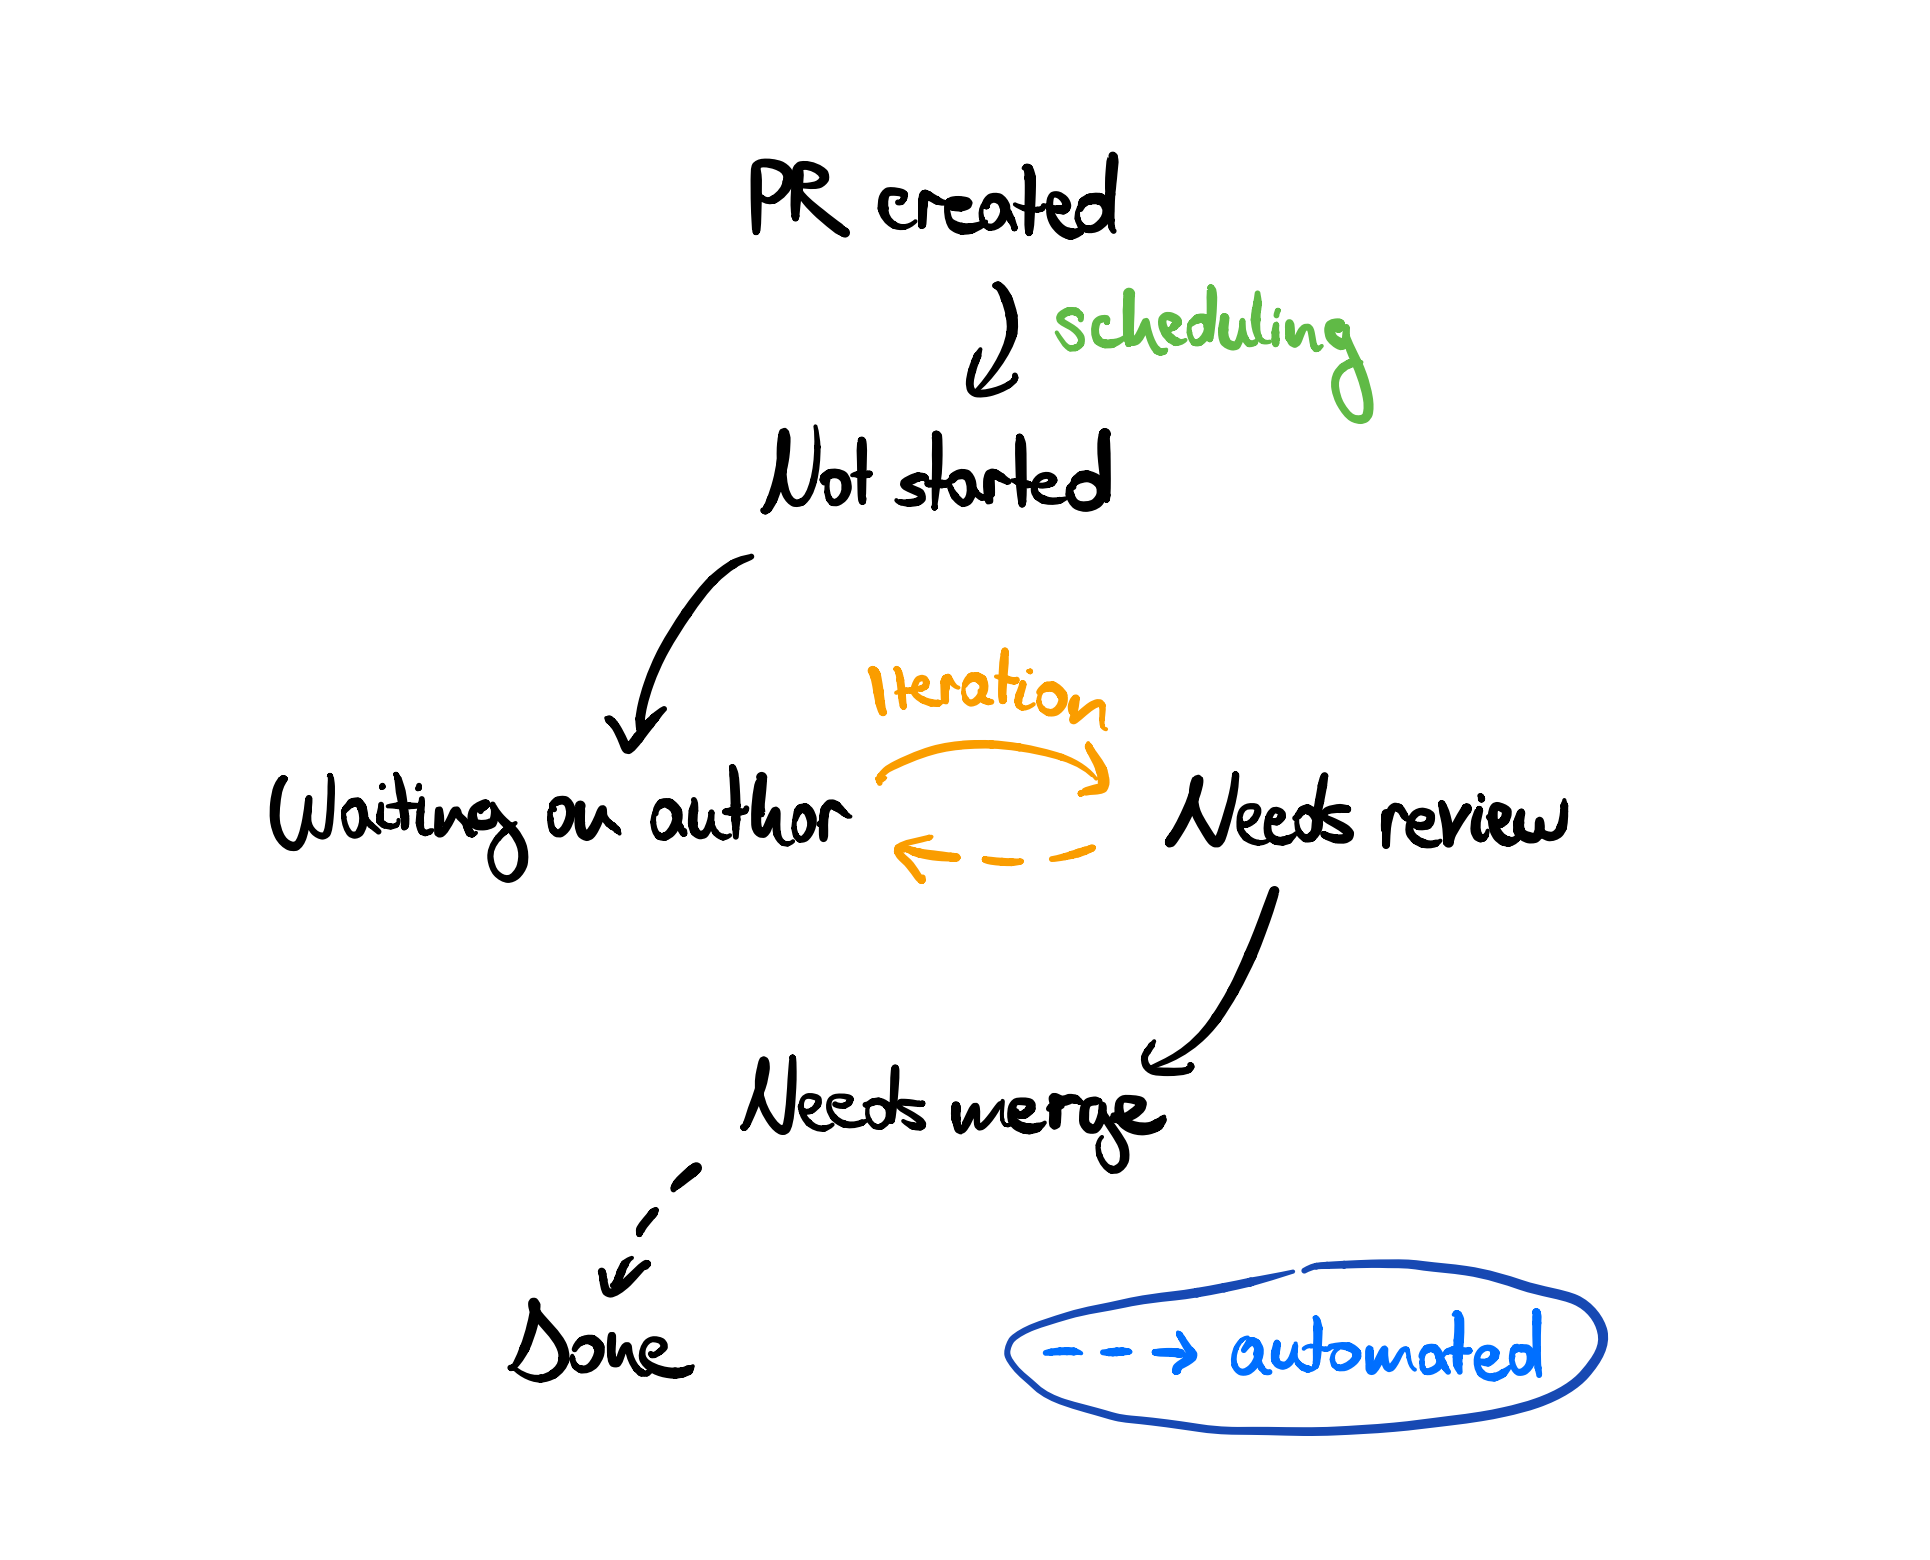
\includegraphics[width=10cm]{images/pr_backlog.png}
\end{frame}

\section{Communication}
\begin{frame}{Terminology}\pause
\begin{itemize}
    \item An issue is \b{approved} once it was confirmed and labeled by a member of the TypeScript team.\pause
    \item An issue is \b{scheduled} (or a milestone bug) once it was assigned to a milestone that is not the \code{Backlog} milestone, like an upcoming release of TypeScript.\pause
    \item An issue is \b{assigned} once it was assigned to a member of the TypeScript team. Commonly all scheduled issues are also assigned. Unscheduled issues are sometimes assigned too, but usually only after a pull request was opened.
\end{itemize}
\end{frame}
\begin{frame}{Quantitative analysis}\pause
\begin{itemize}
    \item A \b{meaningful action} could be either a group of messages, a review, or updating some pull request characteristic like adding a label or moving the pull request within a project board.\pause
    \item The \b{response time} measures the time between meaningful actions.\pause
    \item The \b{immediate response time} measures the time until a meaningful response to an action by me.
\end{itemize}\pause

\padding

Time difference is measured in days.\pause

The results are based on 40 responses.
\end{frame}
\begin{frame}{}
\centering
\begin{tikzpicture}
\begin{axis}[width=10cm,
    height=7cm,
    ybar,
    bar width=0.3cm,
    ylabel={days},
    xtick=data,
    xticklabels from table={\datatable}{A},
    ymajorgrids]
    \addplot table [x expr=\coordindex, y=B]{\datatable};
    \addplot table [x expr=\coordindex, y=C]{\datatable};
    \addplot table [x expr=\coordindex, y=D]{\datatable};
    \legend{$\top$, $I$, $\neg I$}
\end{axis}
\end{tikzpicture}
\centering
Average response time by state \\ ($\top \sim$ any, $S \sim$ scheduled, $A \sim$ assigned, $I \sim$ immediate)
\end{frame}
\begin{frame}{}
\begin{itemize}
    \item The average response time in issues was 2.1 days compared to 6 days in pull requests.\pause
    \item My pull requests were open an average of 30.4 days (assuming open pull requests are closed today).
\end{itemize}
\end{frame}

\section{Feedback}
\begin{frame}{Feedback}
\begin{itemize}
    \item The planning of new features is lacking community involvement.\pause
    \item Mentoring could be featured more prominently.\pause
    \item Improve code structure, documentation, and test suite.\pause
    \item Increase iteration speed by automating more elements of the contributing process.
\end{itemize}
\end{frame}

\begin{frame}{}
\centering
Thank you. \\
Questions?
\end{frame}

\begin{frame}[allowframebreaks]{References}

\printbibliography

\end{frame}

\end{document}
